\documentclass{article}
\usepackage{graphicx}
\usepackage{booktabs}
\usepackage{amsmath}
\usepackage{hyperref}
\usepackage{float}

\title{A Study of Optimization Methods for Full Fine-Tuning of Qwen2.5-0.5B}
\author{ Odilzhon Negmatuloev}
\date{}

\begin{document}

\maketitle

\section{Introduction}

This work presents a study of optimization methods for full fine-tuning of a small language model (SLM), Qwen2.5-0.5B. The study compares three distinct optimization approaches: the widely adopted adaptive optimizer AdamW, the recently proposed matrix-aware optimizer Muon, and the zeroth-order optimizer MeZO.

All experiments are conducted in the regime of full fine-tuning, where all model parameters are updated. This investigation addresses the following research questions:

1. How do AdamW, Muon, and MeZO compare in terms of convergence speed and final training loss?

2. What are the memory and computational trade-offs of each optimizer?

3. Do differences in training dynamics translate to differences in downstream task performance?
\section{Optimization Methods}

\subsection{AdamW}

AdamW~\cite{loshchilov2017adamw} extends the Adam optimizer by 
\emph{decoupling} weight decay from the adaptive gradient update. 
At each training step $t$, given gradient $g_t = \nabla_\theta \mathcal{L}(\theta_t)$, 
the first and second moment estimates are updated as:

\begin{equation}
m_t = \beta_1 m_{t-1} + (1 - \beta_1) g_t
\end{equation}

\begin{equation}
v_t = \beta_2 v_{t-1} + (1 - \beta_2) g_t^2
\end{equation}

\begin{equation}
\hat{m}_t = \frac{m_t}{1 - \beta_1^t}
\end{equation}

\begin{equation}
\hat{v}_t = \frac{v_t}{1 - \beta_2^t}
\end{equation}

\begin{equation}
\theta_{t+1} = \theta_t 
- \eta \frac{\hat{m}_t}{\sqrt{\hat{v}_t} + \epsilon}
- \eta \lambda \theta_t
\end{equation}

where $\eta$ is the learning rate, $\lambda$ is the weight decay coefficient, 
$\beta_1$ and $\beta_2$ are exponential decay rates, and $\epsilon$ is a small constant 
for numerical stability.

Unlike classical $L_2$ regularization applied inside the adaptive update, 
AdamW applies weight decay as a separate multiplicative shrinkage step, 
ensuring that regularization strength is independent of the adaptive scaling 
of gradients.

\subsection{Muon}

Muon (Momentum Orthogonalized by Newton-Schulz)~\cite{moonshot2025moonlight} is a matrix-aware optimizer that applies orthogonalization-based updates to 2D weight matrices while using standard adaptive methods for other parameters. The core innovation lies in preserving spectral properties of weight matrices during optimization.

For matrix parameters $W \in \mathbb{R}^{m \times n}$, Muon computes:

\begin{equation}
W_{t+1} = \text{NewtonSchulz}(W_t - \eta G_t)
\end{equation}

where $G_t$ is the momentum-accumulated gradient and NewtonSchulz$(\cdot)$ denotes the Newton-Schulz orthogonalization procedure. This operation approximately orthogonalizes the update using a Newton–Schulz iteration, helping preserve spectral properties of weight matrices rather than performing an exact projection onto the nearest orthogonal matrix.

\subsection{MeZO}

MeZO (Memory-efficient Zeroth-Order Optimization) \cite{malladi2023mezo}
is based on the classical Simultaneous Perturbation Stochastic Approximation (SPSA) gradient estimator. Unlike first-order methods, MeZO does not rely on backpropagation and instead estimates gradients using forward evaluations only.

Given parameters $\theta \in \mathbb{R}^d$ and a minibatch $\mathcal{B}$, a random perturbation vector $z \sim \mathcal{N}(0, I_d)$ is sampled. The SPSA gradient estimator is:

\begin{equation}
\hat{\nabla}\mathcal{L}(\theta; \mathcal{B}) =
\frac{
\mathcal{L}(\theta + \epsilon z; \mathcal{B})
-
\mathcal{L}(\theta - \epsilon z; \mathcal{B})
}
{2\epsilon}
\, z
\label{eq:spsa}
\end{equation}

where $\epsilon$ is a small perturbation scale. The parameter update is then given by:

\begin{equation}
\theta_{t+1}
=
\theta_t
-
\eta_t
\hat{\nabla}\mathcal{L}(\theta_t; \mathcal{B}_t).
\label{eq:mezo_update}
\end{equation}

Each SPSA estimate requires two forward passes through the model. Unlike standard zeroth-order implementations, which explicitly store the perturbation vector $z$, MeZO uses an in-place implementation that reconstructs $z$ via a fixed random seed. This allows the method to achieve a memory footprint equivalent to inference-time memory, since no gradient tensors or optimizer states are stored.

While MeZO eliminates backward propagation and gradient storage, the gradient estimate has higher variance compared to first-order methods, which may negatively impact convergence stability.

\section{Experimental Setup}

\subsection{Computational Infrastructure}

Experiments were conducted using the following configuration:
\begin{itemize}
    \item \textbf{Hardware:} 2× NVIDIA Tesla T4 GPUs (15 GB VRAM each)
    \item \textbf{Precision:} FP32 (Tesla T4 lacks native BF16 support)
    \item \textbf{Budget constraint:} 30 GPU hours per week
\end{itemize}

The memory and compute limitations of the T4 architecture necessitated careful experimental design and motivated dataset size reduction.

\subsection{Model Architecture}

The base model used is Qwen2.5-0.5B, a 0.5 billion parameter causal language model. All parameters were updated during fine-tuning.

\subsection{Dataset}

Training was performed on OpenWebText-10k, consisting of the first 10,000 examples from the OpenWebText corpus. This subset was selected to accommodate the computational budget while enabling meaningful optimizer comparison.

Text preprocessing followed standard causal language modeling procedures. Documents were tokenized using the model’s native tokenizer, concatenated, and packed into fixed-length sequences of 512 tokens. Sequence packing maximizes GPU utilization by minimizing padding overhead and ensures efficient use of the available context window during training.

\subsection{Training Configuration}

To ensure fair comparison, core hyperparameters were standardized across first-order methods (AdamW and Muon). MeZO required adjusted hyperparameters due to its fundamentally different optimization dynamics.

\textbf{Common settings:}
\begin{itemize}
    \item Sequence length: 512 tokens
    \item Per-device batch size: 2 (gradient accumulation steps: 8; effective batch size: 16)
    \item Learning rate scheduler: Cosine
    \item Precision: FP32
\end{itemize}

\textbf{AdamW and Muon hyperparameters:}
\begin{itemize}
    \item Learning rate: $5 \times 10^{-5}$
    \item Weight decay: 0.05
\end{itemize}

\textbf{MeZO hyperparameters:}
\begin{itemize}
    \item Learning rate: $2 \times 10^{-5}$
    \item Zo-eps: $1 \times 10^{-3}$
    \item Weight decay: 0.0
    \item Perturbation parameter: $\epsilon = 10^{-3}$
\end{itemize}

The lower learning rate and zero weight decay for MeZO were determined through preliminary experiments and align with recommendations in the original work.

\subsection{Evaluation Methodology}

Models were evaluated using the EleutherAI Language Model Evaluation Harness on five commonsense reasoning benchmarks in zero-shot setting:

\begin{itemize}
\item \textbf{PIQA}: Physical interaction question answering
\item \textbf{ARC-Easy}: Elementary-level science questions
\item \textbf{ARC-Challenge}: Complex science questions
\item \textbf{Winogrande}: Pronoun resolution requiring commonsense reasoning
\item \textbf{HellaSwag}: Sentence completion with commonsense inference
\end{itemize}

\section{Implementation Details}

\subsection{Muon Integration}

The Muon optimizer was integrated from the Moonlight repository~\cite{moonshot2025moonlight} as a standard \texttt{torch.optim.Optimizer} subclass. Integration required minimal modification: the optimizer class was incorporated into the codebase and instantiated via the \texttt{create\_optimizer} method of Hugging Face's \texttt{Trainer}.

Two Muon-based configurations were evaluated. In the \textbf{pure Muon} setting, Muon was applied to all 2D weight matrices (229,638,144 parameters, 59.60\% of total parameters), while the remaining parameters were left unchanged. In the \textbf{hybrid Muon+AdamW} configuration, Muon was applied to the same subset of matrix parameters (59.60\%), and the remaining 155,644,928 parameters (40.40\%) were optimized using AdamW.

The original implementation includes the following caveats:

\begin{itemize}
\item ``We believe it may not work well for finetuning pretrained models.''
\item ``We believe this optimizer is unlikely to work well with small batch sizes.''
\end{itemize}

\subsection{MeZO Implementation}

The MeZO implementation was adapted from the original repository~\cite{malladi2023mezo}. Due to dependency conflicts and deprecated API usage in the original codebase, core algorithmic components were extracted and reimplemented within a modern \texttt{transformers.Trainer} framework.

A custom \texttt{MeZOTrainer} class was developed, inheriting from \texttt{transformers.Trainer} and overriding the training loop. Key functions—\texttt{zo\_step} (gradient estimation), \texttt{zo\_update} (parameter update), and \texttt{\_perturb\_parameters}—were ported with minimal modifications to ensure algorithmic fidelity while maintaining compatibility with current library versions.

\section{Results}

\subsection{Training Dynamics}
Figure~\ref{fig:loss_comparison} presents training loss trajectories, and Table~\ref{tab:loss_stats} summarizes key statistics.

\begin{figure}[H]
    \centering
    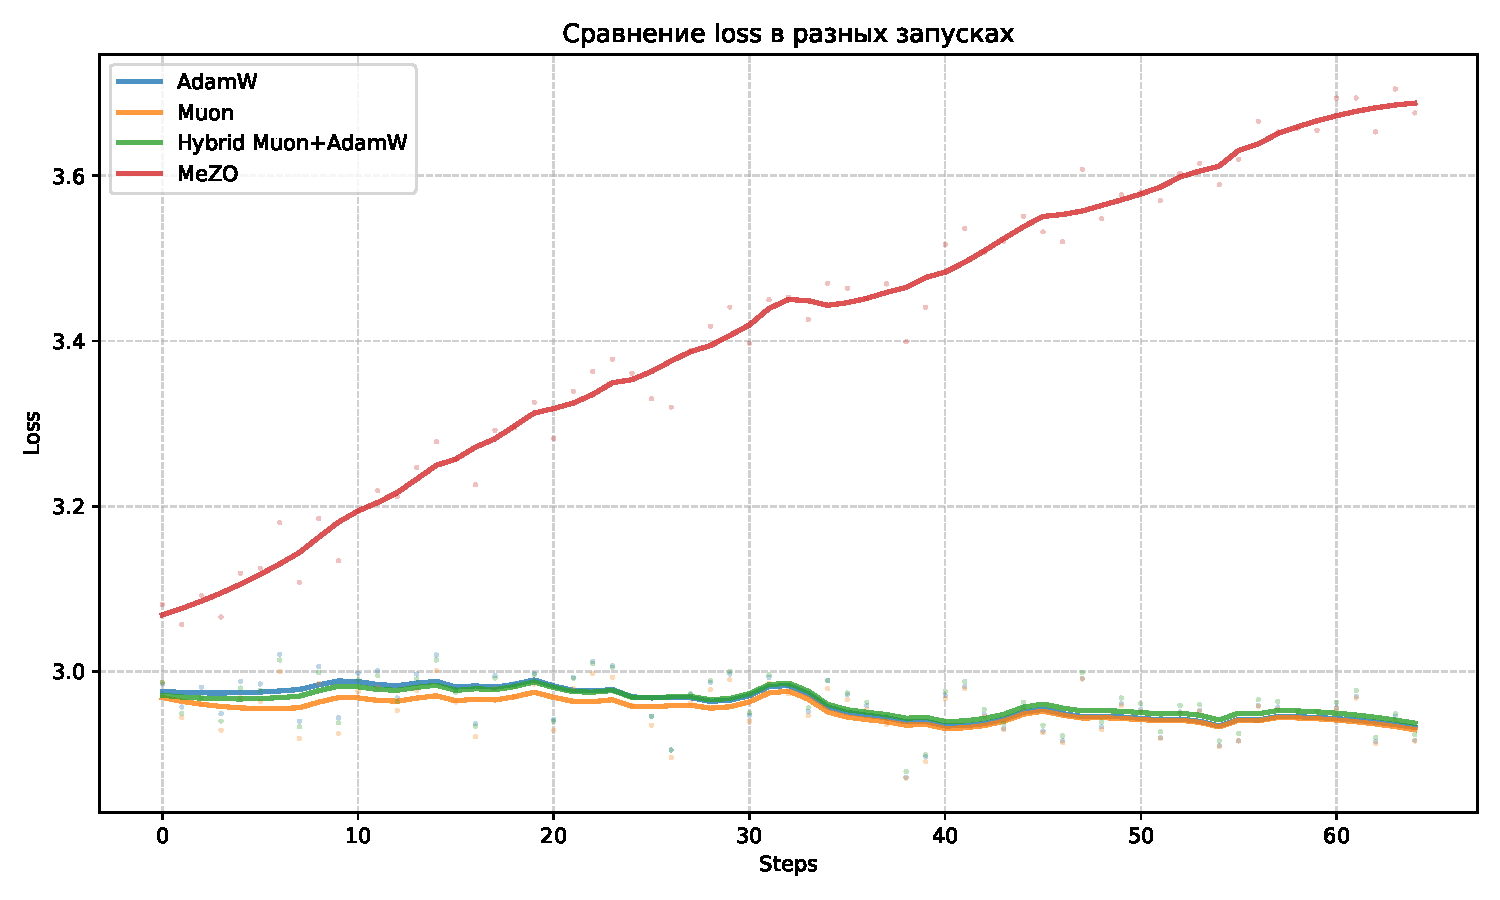
\includegraphics[width=0.95\linewidth]{loss_comparison.pdf}
    \caption{Training loss curves across optimizers. AdamW and Muon exhibit nearly identical convergence trajectories, while MeZO shows substantially higher loss and increased instability.}
    \label{fig:loss_comparison}
\end{figure}



\begin{table}[h]
\centering
\begin{tabular}{lcccc}
\toprule
\textbf{Optimizer} & \textbf{Initial} & \textbf{Min} & \textbf{Max} & \textbf{Final} \\
\midrule
AdamW & 2.985 & 2.872 & 3.020 & 2.916 \\
Muon & 2.987 & 2.871 & 3.000 & 2.915 \\
Hybrid Muon+AdamW  & 2.987 & 2.878 & 3.014 & 2.923 \\
MeZO  & 3.080 & 3.057 & 3.705 & 3.675 \\
\bottomrule
\end{tabular}
\caption{Training loss statistics. Best values in bold.}
\label{tab:loss_stats}
\end{table}

\textbf{Key observations:}
\begin{itemize}
    \item AdamW, Muon, Hybrid Muon+AdamW demonstrate nearly identical convergence behavior
    \item MeZO exhibits substantially degraded performance: final loss 26\% higher than AdamW, with pronounced instability (max loss 3.705 vs 3.020 for AdamW).
\end{itemize}

\subsection{Computational Efficiency}

Table~\ref{tab:efficiency} presents training efficiency metrics.

\begin{table}[h]
\centering
\begin{tabular}{lccc}
\toprule
\textbf{Optimizer} & \textbf{Final Loss} & \textbf{Time (hrs)} & \textbf{Peak Memory (GB)} \\
\midrule
AdamW & 2.916 & 2.5 & 8.705 \\
Muon  & 2.915 & 3.2 & 7.660 \\
Hybrid Muon+AdamW  & 2.923 & 3 & 8.240 \\
MeZO  & 3.675 & 1.7 & 7.479 \\
\bottomrule
\end{tabular}
\caption{Training efficiency comparison. Peak memory refers to GPU$_0$ maximum usage.}
\label{tab:efficiency}
\end{table}


\begin{itemize}
    \item \textbf{Muon} reduces peak memory usage by approximately 12.0\% relative to AdamW (7.660 GB vs 8.705 GB), reflecting its reduced optimizer state footprint for matrix parameters.
    
    \item \textbf{Hybrid Muon+AdamW} achieves a smaller memory reduction of approximately 5.3\% (8.240 GB vs 8.705 GB), consistent with only 59.6\% of parameters being optimized with Muon.
    
    \item \textbf{MeZO} achieves the lowest memory footprint (7.479 GB), corresponding to a 14.1\% reduction relative to AdamW. This aligns with its gradient-free design, which avoids storing first- and second-moment optimizer states.
\end{itemize}

\subsection{Downstream Task Performance}

Table~\ref{tab:downstream} presents zero-shot accuracy on five commonsense reasoning benchmarks. In addition to per-task results, we report the average accuracy across tasks and the difference relative to the base pretrained model.

\begin{table*}[t]
\centering
\small
\begin{tabular}{lcccccc}
\toprule
\textbf{Model} 
& \textbf{PIQA} 
& \textbf{ARC-E} 
& \textbf{ARC-C} 
& \textbf{Winogrande} 
& \textbf{HellaSwag}
& \textbf{Avg} \\
\midrule
Base (Qwen2.5-0.5B) 
& 0.7051 
& 0.6465 
& 0.2910 
& 0.5643 
& 0.4059 
& 0.5226 
& -- \\
\midrule
AdamW & 0.7035 & 0.6667 & 0.2961 & 0.5683 & 0.3982 & 0.5266 \\
Muon  & 0.7029 & 0.6654 & 0.2909 & 0.5674 & 0.3989 & 0.5251 \\
Muon+AdamW  & 0.7013 & 0.6671 & 0.3003 & 0.5596 & 0.4006 & 0.5258 \\
MeZO  & 0.6382 & 0.5370 & 0.2619 & 0.5351 & 0.3592 & 0.4663 \\
\bottomrule
\end{tabular}
\caption{Zero-shot accuracy on downstream tasks. Average (Avg) is computed across the five benchmarks.}
\label{tab:downstream}
\end{table*}

\textbf{Key findings:}
\begin{itemize}
    \item AdamW, Muon, Hybrid Muon+AdamW achieve nearly identical average performance (0.5266 vs 0.5251), with absolute differences below 0.002 accuracy, indicating practical equivalence under the current setup.
    
    \item Compared to the base pretrained model (0.5226 average accuracy), fine-tuning with AdamW and Muon yields a very small improvement (+0.002 to +0.004). Given the reported standard errors of individual tasks (≈0.005–0.014), these differences fall within expected statistical variation and should not be interpreted as meaningful gains.
    
    \item MeZO underperforms substantially, showing a 5.6 percentage point drop relative to the base model, consistent across all tasks and aligned with its degraded training convergence.
\end{itemize}

Downstream differences among AdamW, Muon, and Hybrid Muon+AdamW remain negligible. While MeZO exhibits clear degradation. The marginal improvements over the base model suggest that short-horizon full fine-tuning on a 10k subset provides limited task-level benefit in this regime.

\section{Discussion}

\subsection{AdamW vs Muon: Comparable Performance with Reduced Memory}

The experimental results indicate that Muon achieves practical performance parity with AdamW in both training dynamics and downstream benchmark accuracy. Final training losses differ by less than 0.001, and average downstream accuracy differs by less than 0.002 absolute points—well within the reported task-level standard errors.

In terms of memory efficiency, the pure Muon configuration reduces peak GPU memory usage by approximately 12\% relative to AdamW (7.66 GB vs 8.71 GB). The hybrid Muon+AdamW configuration yields a smaller reduction of approximately 5.3\%, consistent with only 59.6\% of parameters being optimized using Muon.

Overall, within the current small-scale fine-tuning regime, Muon provides measurable memory savings without observable degradation in optimization stability or downstream performance. However, given the limited dataset size and single-epoch training setup, these results should be interpreted as evidence of equivalence under constrained conditions rather than proof of general optimizer superiority.

\subsection{MeZO: Memory Efficiency at the Cost of Convergence Quality}

MeZO delivers on its promise of reduced memory consumption (14.1\% reduction), making it potentially valuable for extremely memory-constrained scenarios. However, this comes at substantial cost:

\begin{itemize}
    \item \textbf{Convergence degradation:} Final training loss 26\% higher than first-order methods
    \item \textbf{Downstream performance gap:} 11.4\% lower average accuracy than AdamW
\end{itemize}


\subsection{Limitations}

Several experimental constraints limit the generalizability of these findings:

\begin{itemize}
    \item \textbf{Dataset size:} The 10k-example subset may not reflect behavior on full-scale corpora.
    \item \textbf{Training duration:} 1 epoch (658 steps) represents early-stage fine-tuning; longer training may reveal different optimizer characteristics.
    \item \textbf{Hardware constraints:} FP32 precision on T4 GPUs differs from typical BF16/FP16 training on modern accelerators.
\end{itemize}

\section{Conclusion}

This study provides a controlled empirical comparison of three optimization methods for full fine-tuning of the Qwen2.5-0.5B language model. The key findings are:

\begin{enumerate}
    \item \textbf{Convergence Speed and Final Training Loss.}  
    AdamW and pure Muon exhibit nearly identical convergence dynamics, with final training losses differing by less than 0.001. The hybrid Muon+AdamW configuration shows similarly close behavior. Within the single-epoch, small-batch regime considered here, no meaningful difference in optimization quality can be established between first-order methods. In contrast, MeZO demonstrates substantially degraded convergence, with approximately 26\% higher final loss and increased instability.
    
    \item \textbf{Memory and Computational Trade-offs.}  
    Pure Muon reduces peak GPU memory usage by approximately 12\% relative to AdamW, while the hybrid Muon+AdamW configuration yields a smaller reduction of approximately 5.3\%. MeZO achieves the largest memory reduction (14.1\%), reflecting its gradient-free design. However, this gain comes at the cost of significantly degraded optimization performance, illustrating a clear trade-off between memory efficiency and convergence reliability in the evaluated regime.

    \item \textbf{Downstream Task Performance.}  
    AdamW and Muon achieve nearly identical downstream benchmark accuracy, with average differences below 0.002 absolute points—well within reported task-level standard errors. Fine-tuning yields only marginal improvements over the base pretrained model, suggesting limited task-level adaptation in this short-horizon setting. In contrast, MeZO exhibits a consistent and substantial performance drop across benchmarks.
\end{enumerate}

Overall, within the constraints of the current experimental setup, AdamW remains the most reliable choice, with Muon serving as a promising memory-efficient alternative that maintains comparable performance. The substantial memory savings achieved by MeZO come at too high a cost in optimization quality, making it impractical for standard fine-tuning scenarios. At the same time, a fair assessment of its capabilities requires reproducing the experimental conditions described in the original paper, as the present configuration may not reflect the regime in which MeZO demonstrates its claimed advantages.

Further research with larger batch sizes and more extensive datasets is necessary to better understand the true potential and limitations of both Muon and MeZO.


\bibliographystyle{plain}
\begin{thebibliography}{99}

\bibitem{loshchilov2017adamw}
I.~Loshchilov and F.~Hutter.
\newblock Decoupled weight decay regularization.
\newblock In \textit{International Conference on Learning Representations (ICLR)}, 2019.

\bibitem{moonshot2025moonlight}
MoonshotAI.
\newblock Moonlight: Muon Optimizer for Scalable LLM Training.
\newblock GitHub repository, 2025.
\newblock \url{https://github.com/MoonshotAI/Moonlight}

\bibitem{malladi2023mezo}
S.~Malladi, T.~Gao, E.~Nichani, A.~Damian, J.~D.~Lee, D.~Chen, and S.~Arora.
\newblock Fine-tuning language models with just forward passes.
\newblock In \textit{Advances in Neural Information Processing Systems (NeurIPS)}, 2023.
\newblock \url{https://github.com/princeton-nlp/MeZO}

\end{thebibliography}

\end{document}